\documentclass[../main.tex]{subfiles}
\graphicspath{{\subfix{../figures/}}}

\begin{document}
    Zunächst wird ein einfaches Szenario betrachtet: Ein neuer Erreger tritt erstmals auf, wobei eine geringe Zahl von Infizierten in eine vollständig suszeptible Bevölkerung eingeführt wird.
    Ein grundlegendes Problem besteht dann in der Modellierung der weiteren epidemischen Ausbreitung.
    Dafür eignet sich das SIR-Modell, welches auf eine Arbeit von Kermack und McKendrick aus dem Jahr 1927 zurückgeht (vgl. \cite[S. 90]{Bri03}).

    \subsection{Mathematische Ansätze}
    \label{ssec:mathematical_approach}
    Folgende Konzepte finden in epidemiologischen Modellen verbreitet Anwendung:
        \subsubsection{Einteilung der Population in Gruppen}
        \label{sssec:compartments}
        Die Bevölkerung der Gesamtzahl $N$ wird in sogenannte \glqq compartments\grqq\  aufgeteilt, die im Bezug auf die Krankheit unterschiedliche Eigenschaften aufweisen und nach  Bedarf definiert werden können. Folgende Gruppen werden im SIR-Modell verwendet und bilden die Grundlage für komplexere Modelle (vgl. \cite[S. 2]{Sul12}):

        \begin{description}
            \item[S] (engl.: \textit{susceptible}) Empfängliche Individuen, die von $I$ mit der Krankheit infiziert werden können.
            \item[I] (engl.: \textit{infectious}) Infizierte Individuen, die die Krankheit an $S$ weitergeben können.
            \item[R] (engl.: \textit{removed}) Individuen, die aufgrund von Immunität nach Genesung oder Impfung, Tod oder Isolation nicht infiziert werden können.
        \end{description}
        Es gilt:
        \begin{equation}
            \label{eq:constant_population}
            N = S + I + R
        \end{equation}

        Jedes Individuum befindet sich zu jedem Zeitpunkt in genau einer dieser Gruppen. Insgesamt kann so der momentane Krankheitszustand in der Bevölkerung durch die Anzahl von Individuen in der jeweiligen Gruppe angegeben werden.

        \subsubsection{Zeitliche Veränderung der Gruppen durch Übergänge}
        \label{sssec:transitions}

        Das Ziel des Modells besteht darin, die Anzahl von Individuen in allen definierten Gruppen zu jedem Zeitpunkt zu kennen. 
        Dafür muss der Wechsel von Individuen zwischen Gruppen mithilfe von Übergängen modelliert werden.
        
        Das Schema, nach welchem die Gruppen im SIR-Modell durchlaufen werden, kann in einem Transferdiagramm (Abbildung \ref{fig:sir_transfer_verbose}) dargestellt werden. Die Bezeichnung als SIR-Modell resultiert dabei aus der Reihenfolge, nach der die Gruppen durchlaufen werden.
        Jeder Pfeil im Transferdiagramm entspricht einem Übergang in die entsprechende Richtung. Dabei wird aus der Ausgangsgruppe des Pfeils die Anzahl von Individuen entfernt, welche der Zielgruppe hinzugefügt wird.

        \begin{figure}[h]
            \centering
            \begin{tikzpicture}
            \tikzmath{\bl=1.5; \al=3;} %bl:boxlength, al:arrowlength
            \tikzmath{\bl=1.5; \al=3;}
                \foreach \t\n in {S/0, I/1, R/2}
                \tikzmath{\x = \n*\bl + \n*\al;}
                \draw (\x, 0) rectangle node{\t} (\x+\bl, \bl);

                \foreach \t\n in {Infektion/0, Genesung/1}
                    \tikzmath{\x = \bl + \n*\bl + \n*\al;}
                    \draw[-{>[scale=2]}] (\x, 0.5*\bl) -- node[auto]{\t} (\x+\al, 0.5*\bl);
            \end{tikzpicture}
            \caption{Anschauliches Transferdiagramm: SIR-Modell}
            \label{fig:sir_transfer_verbose}
        \end{figure}


        Bei der Größe der Gruppen handelt es sich um zeitabhängige Funktionen $S(t)$, $I(t)$ und $R(t)$. Da es schwierig ist, diese Funktionen direkt zu bestimmen, wird zunächst die Veränderung innerhalb eines kurzen Zeitraums betrachtet (vgl. \cite[S. 7]{Li18}).
        Demnach gilt für die Änderung einer Gruppe $X$ über die Dauer $\Delta t$:
        \begin{equation}
            \label{eq:difference}
            \begin{split}
                \Delta X &= X(t+\Delta t) - X(t) \\
                         &= X_{in} - X_{out}
            \end{split}
        \end{equation}

        Diese Änderung entspricht der Differenz aus während $\Delta t$ eintretender Individuen $X_{in}$ und verlassender Individuen $X_{out}$ (vgl. \cite[S. 7]{Li18}).
        Für das SIR-Modell erhalten wir folgende Differenzengleichungen:
        \begin{equation}
            \label{eq:sir_difference_verbose}
            \setlength{\jot}{10pt}
            \begin{aligned}
            \Delta S(t) &= -\fbox{Neuinfektionen}, \\
            \Delta I(t) &= \fbox{Neuinfektionen} - \fbox{Genesungen}, \\
            \Delta R(t) &= \fbox{Genesungen}
            \end{aligned}
        \end{equation}


        Es gilt also, einen mathematischen Ausdruck für die Anzahl von Neuinfektionen und Genesungen zu finden. Jeder Übergang stellt grundsätzlich ein Produkt aus dem betrachteten Zeitintervall sowie folgenden möglichen Faktoren dar:
        \begin{equation*}
            \fbox{Rate} \cdot \fbox{Wahrscheinlichkeit} \cdot \fbox{Gruppe} \cdot \Delta t
        \end{equation*}
        
        \paragraph{Neuinfektionen} werden durch den Term
        \begin{equation*}
            \beta \cdot \frac{S}{N} \cdot I \cdot \Delta t
        \end{equation*}
        ausgedrückt, der interpretiert werden kann als:
        \begin{equation*}
            \fbox{\parbox{4cm}{Anzahl effektiver Kontakte eines Infizierten pro Tag}}
            \cdot
            \fbox{\parbox{4cm}{Wahrscheinlichkeit des Kontaktes mit einem Suszeptiblen}}
            \cdot
            \fbox{\parbox{2cm}{Anzahl \\Infizierter}}
            \cdot
            \Delta t
        \end{equation*}
        Bei dieser Form der Inzidenz, also der Häufigkeit von Neuinfektionen, wird die Kontaktrate $\beta$ als unabhängig von der Bevölkerungsdichte betrachtet. Sie wird als Standardinzidenz bezeichnet und eignet sich für die Modellierung menschlicher Krankheiten (vgl. \cite[S. 602]{Het00}).

        \paragraph{Genesungen} werden durch den Term
        \begin{equation*}
            \gamma \cdot 1 \cdot I \cdot \Delta t
        \end{equation*}
        ausgedrückt, der interpretiert werden kann als:
        \begin{equation*}
            \fbox{\parbox{3cm}{Anteil der pro Tag genesenden Infizierten}}
            \cdot
            \fbox{\parbox{4cm}{Genesung erfolgt sicher mit Wahrscheinlichkeit von 100\%}}
            \cdot
            \fbox{\parbox{2cm}{Anzahl \\Infizierter}}
            \cdot
            \Delta t
        \end{equation*}
        Diese Terme können in die Differenzengleichungen \eqref{eq:sir_difference_verbose} eingesetzt werden:
        \begin{equation}
            \label{eq:sir_difference}
            \setlength{\jot}{0.4cm}
            \begin{aligned}
            \Delta S(t) &= - \frac{\beta}{N} S I \cdot \Delta t \\
            \Delta I(t) &= \frac{\beta}{N} S I \cdot \Delta t - \gamma I \cdot \Delta t \\
            \Delta R(t) &= \gamma I \cdot \Delta t
            \end{aligned}
        \end{equation}

        Als Maß für die zeitliche Änderung der Gruppen liegt die Verwendung der Ableitungen $S'(t)$, $I'(t)$ und $R'(t)$ nahe. Anstatt der in in System \eqref{eq:sir_difference} verwendeten absoluten Änderungen benötigen wir dann die Änderungsraten, welche sich über Division durch $\Delta t$ und die Grenzwertbetrachtung $\Delta t \to 0$ ergeben (vgl. \cite[S. 7]{Li18}):
        \begin{equation}
            \label{eq:differential}
            \lim \limits_{\Delta t \to 0} \frac{\Delta X}{\Delta t}
            = \lim \limits_{\Delta t \to 0} \frac{X(t+\Delta t) - X(t)}{\Delta t}
            = X'(t)
        \end{equation}
  
    \subsection{Vorstellung der Annahmen}
    \label{ssec:assumptions1}
    Die in dieser Arbeit genutzten Modelle beruhen auf folgenden allgemeinen Annahmen (vgl. \cite[S. 8f]{Li18}):
    \begin{itemize}
      \item Die Population weist eine homogene Struktur auf .

      Dies stellt die größte Einschränkung dar, da folglich weder räumliche Dynamiken noch Altersstruktur berücksichtigt werden. Das Alter beeinflusst jedoch maßgeblich das Kontaktverhalten und den Krankheitsverlauf.
      Da zu Beginn der Ausbreitung wenige Infektionen lokal begrenzt auftreten, kann das Modell in dieser ersten Phase nicht genutzt werden (vgl. \cite[S. 25]{Bra08}).

      \item Die Größe der Gruppen wird als differenzierbare Funktion betrachtet. Dies ist erforderlich, da die zugehörige Änderungsrate durch die erste Ableitung beschrieben wird (vgl. \cite[S. 25]{Bra08}).
      
      Daraus folgt, dass das Modell keine diskreten Werte liefert. Da die Bevölkerungszahl in Deutschland jedoch entsprechend groß ist, stellen kontinuierliche Werte keine bedeutende Einschränkung dar.
      Da auch zufallsmäßige Abweichungen in einer großen Population vernachlässigt werden können, ist diese deterministische Betrachtungsweise angemessen.
      
      \item Es erfolgt keine Modellierung der demographischen Dynamik, sodass Geburten und Todesfälle vernachlässigt werden. Da es sich um ein geschlossenes System handelt, aus dem weder Individuen entfernt noch von außen hinzugefügt werden, bleibt die Population gemäß Gleichung \eqref{eq:constant_population} konstant.

      Diese Annahme ist sinnvoll, da der Zeitraum der Modellierung gegenüber der Lebenserwartung eines Individuums gering ist.
    \end{itemize}

    Zudem werden Annahmen bezüglich der Krankheit und ihrer Übertragung getroffen (vgl. \cite[S. 8f]{Li18}, \cite[S. 12]{Sul12}). Sie lauten für das SIR-Modell:

    \begin{itemize}
      \item Infektionen erfolgen über direkten Kontakt zwischen Suszeptiblen und Infizierten. Die Anzahl dieser Kontakte ist direkt proportional zur Anzahl von Suszeptiblen und Infektiösen.
      Die Infektionsrate besitzt daher die Form $\lambda S I$, wobei $\lambda = \frac{\beta}{N}$.

      \item Die Infektiosität beginnt ohne Latenzzeit mit dem Zeitpunkt der Infektion.
      
      \item Eine überstandene Infektion führt zu dauerhafter Immunität. Reinfektion ist damit ausgeschlossen.

      \item Die Genesungsrate ist proportional zur Anzahl der Infizierten und durch $\gamma I$ gegeben.
      
      Der Vorgang der Genesung ist bei genauerer Betrachtung ein mögliches Szenario für das Verlassen einer Gruppe nach einer bestimmten Aufenthaltsdauer. Solche Übergänge werden grundsätzlich als Produkt aus einer Konstanten und der Ausgangsgruppe modelliert, wobei die Konstante die Inverse der Aufenthaltszeit $\tau$ darstellt: $\gamma = \frac{1}{\tau}$. Im Anwendungsbeispiel ergibt sich für eine Dauer der Infektiosität $\tau$ von 10 Tagen: $\gamma=\frac{1}{10}$.
      Bei einer Infektionsdauer $\tau$ verlässt gemäß obigem Ausdruck also pro Zeiteinheit der Anteil $\frac{1}{\tau}$ die Ausgangsgruppe. Dies widerspricht der Vorstellung einer konstanten Aufenthaltszeit, reduziert jedoch die Komplexität des Modells. Es kann gezeigt werden, dass dieser Ansatz zu einer Exponentialverteilung der Aufenthaltszeit mit dem Durchschnittswert $\tau = \frac{1}{\gamma}$ führt (vgl. \cite[S. 88]{Bri03}, \cite[S. 14]{Li18}).

    \end{itemize}

    \subsection{Definition des Modells}
    \label{ssec:definition1}

    Zur Bestimmung der Ableitungen wird die rechte Seite der Differenzengleichungen \eqref{eq:sir_difference} nun für $\Delta X$ in Gleichung \eqref{eq:differential} eingesetzt.
    Es entsteht ein Differentialgleichungssystem \eqref{eq:sir} der ersten Ordnung, das einen Zusammenhang zwischen den Funktionen, das heißt den Größen der Gruppen, und deren Ableitungen herstellt (vgl. \cite[S. 713]{KM27}):
    \begin{equation}
      \label{eq:sir}
      \setlength{\jot}{0.5cm}
      \begin{aligned}
        \frac{dS}{dt} &= - \frac{\beta}{N} S I, \\
        \frac{dI}{dt} &= \frac{\beta}{N} S I - \gamma I, \\
        \frac{dR}{dt} &= \gamma I
      \end{aligned}
    \end{equation}
    Es gelten folgende Anfangsbedingungen:
    \begin{equation*}
        \begin{aligned}
        &S(0) = S_0 \geq 0, \\
        &I(0) = I_0 \geq 0, \\
        &R(0) = R_0 = 0
        \end{aligned}
    \end{equation*}
    
    Wir halten fest, dass das System im Modell durch seine Veränderung beschrieben wird.
    Die Differentialgleichungen sind gewöhnlich, da die Zeit die einzige unabhängige Variable darstellt und autonom, da sie nicht explizit von der Zeit abhängen (vgl. \cite[S. 41f, 534]{Heu13}).
    Dadurch beschreibt \eqref{eq:sir} ein deterministisches, dynamisches System, dessen Zustand sich mit der Zeit ändert.
    Die Entwicklung ist dabei nur vom Anfangszustand und den Regeln des Modells abhängig (vgl. \cite[S. 25]{Bra08}).

    Die Lösung einer Differentialgleichung besteht nun nicht wie gewohnt in einer Variable, sondern einer Funktion. Das Ziel ist daher, die Funktionen $S(t)$, $I(t)$ und $R(t)$ zu bestimmen.

    \subsection{Numerische Lösung des Modells}
    \label{ssec:simulation1}
    Obgleich für das SIR-Modell \eqref{eq:sir} keine geschlossene analytische Lösung existiert (vgl. \cite[S.93]{Bac11}), kann mit dem Euler-Verfahren eine numerische Lösung bestimmt werden.
    
    Bei diesem handelt es sich um das einfachste Verfahren zur Lösung von Anfangsproblemen der Form:
    \begin{equation*}
        \begin{aligned}
            &X' = f(X), &X_0 = X(t_0)
        \end{aligned}
    \end{equation*}

    Im Anwendungsbeispiel entspricht $f$ einem Differentialgleichungssystem und der eingesetzte Wert $X$ einem Vektor aus den Gruppengrößen.
    Der Definitionsbereich wird dabei in kurze diskrete Zeitintervalle der Schrittweite $h$ eingeteilt, welche nacheinander abgegangen werden. An jedem Punkt $X_n$ gibt $f(X_n)$ die Änderungsrate an, sodass sich der momentane Zustand über $h$ um $hf(X_n)$ ändert (vgl. \cite[S. 53]{Heu13}).
    
    Das Euler-Verfahren wird somit durch folgende Iterationsvorschrift ausgedrückt:
    \begin{equation*}
        X_{n+1} = X_n + h f(X_n)
    \end{equation*}

    Dadurch ergeben sich eine oder mehrere Lösungskurven, im Fall des SIR-Modells also die gesuchten Funktionen $S(t)$, $I(t)$ und $R(t)$. Bei dieser Lösung handelt es sich um eine Annäherung, deren Genauigkeit durch die Wahl einer kleineren Schrittweite steigt (vgl. \cite[S. 55]{Heu13}). 
    Zeichnet man die Funktionsgraphen, indem die ermittelten Punkte verbunden werden, so entsteht der klassische Verlauf des SIR-Modells (Abbildung \ref{fig:sir}).

    \begin{figure}[h]
        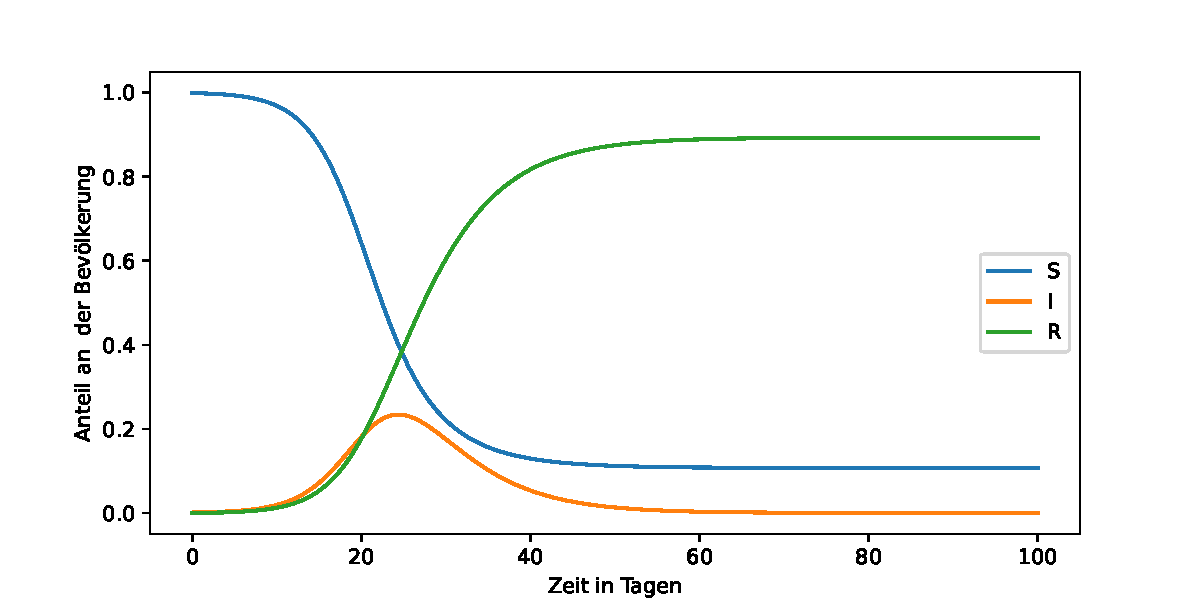
\includegraphics[width=\textwidth]{sir}
        \caption[Verlauf des SIR-Modells]{Verlauf des SIR-Modells mit den Anfangsbedingungen $S=99$, $I=1$, $R=0$ und den Parametern $\beta=0.5$, $\gamma=0.2$}
        \label{fig:sir}
    \end{figure}

    \subsection{Analyse des Modells}
    \label{ssec:analysis1}
    Einige Eigenschaften der Lösung können jedoch auch analytisch einfach festgestellt werden.

    Es existiert eine Lösung für $t \in [0; \infty[$, da die Funktionen gemäß Annahme differenzierbar sind. Diese Lösung ist eindeutig, da der Verlauf eines dynamischen Systems durch seine Anfangsbedingungen festgelegt ist.
    Es kann zudem gezeigt werden, dass die Lösung nicht negativ werden kann, sodass System \eqref{eq:sir} durch Existenz, Eindeutigkeit und Nonnegativität seiner Lösung \glqq well posed\grqq, das bedeutet korrekt gestellt ist (vgl. \cite[S. 37f]{Li18}).

    \paragraph{Die Bevölkerung ist konstant}
    \begin{equation*}
        \begin{split}
            N' & = S' + I' + R' \\
               & = (- \frac{\beta}{N} S I) + (\frac{\beta}{N} S I - \gamma I) + (\gamma I) \\
               & = 0
        \end{split}
    \end{equation*}
    Die Summe der drei Ableitungen ergibt null und damit auch die Änderungsrate der Gesamtbevölkerung, sodass gilt:
    \begin{equation}
        N(t) \forall t \equiv N_0 \coloneqq S_0 + I_0
    \end{equation}

    Folglich bietet es sich an, das System zu normalisieren und statt der absoluten Anzahl von Individuen, deren Anteil an der Gesamtbevölkerung zu verwenden (vgl. \cite[S. 90]{Bri03}). Wir definieren die relative Anzahl an Individuen pro Gruppe, welche Werte im Intervall $[0;1[$ annehmen kann, wie folgt:
    \begin{equation}
        \label{eq:proportions}
        \begin{aligned}
            s &= \frac{S}{N}, & i &= \frac{I}{N}, & r &= \frac{R}{N}
        \end{aligned}
    \end{equation}
    Über diese erhalten wir folgendes normalisiertes System\footnote{Rechenweg im Anhang (S. \pageref{ap:normalization})}:
    \begin{equation}
        \label{eq:sir_norm}
        \begin{aligned}
          \frac{ds}{dt} &= - \beta s i, \\
          \frac{di}{dt} &= \beta s i - \gamma i, \\
          \frac{dr}{dt} &= \gamma i
        \end{aligned}
    \end{equation}


        \subsubsection{Die Reproduktionszahl}
        \label{sssec:reproduction_number}
        Die wichtigste Größe der Epidemiologie ist die Basisreproduktionszahl $R_0$. Sie ist definiert als die Anzahl von sekundären Infektionen, die ein erster Infizierter während der Dauer seiner Infektiosität in einer vollständig suszeptiblen Bevölkerung verursacht (vgl. \cite[S. 161]{DHB13}).

        Es handelt sich um keine biologische Konstante. Ihr Wert ist umweltbedingt und wird wie folgt ausgedrückt (vgl. \cite[S. 1]{Jon07}):
        \begin{equation}
            \label{eq:basic_reproductive_number}
            \begin{split}
                R_0 &= \frac{\beta}{\gamma} s_0 \\
                    &= \beta \cdot \frac{1}{\gamma} \cdot s_0
            \end{split}
        \end{equation}
        Die Basisreproduktionszahl kann als Produkt aus folgenden Faktoren interpretiert werden (vgl. \cite[S. 32]{Li18}):
        \begin{equation*}
            \fbox{\parbox{4cm}{Anzahl effektiver Kontakte eines Infizierten pro Tag}}
            \cdot
            \fbox{\parbox{3cm}{Dauer der Infektiosität in Tagen}}
            \cdot
            \fbox{\parbox{4cm}{Anteil der Suszeptiblen in der Bevölkerung}}
        \end{equation*}

        Durch Umstellung dieser Formel erhalten wir einen Wert für $\beta$:
        \begin{equation*}
            \beta   = \frac{R_0 \cdot \gamma}{s_0}
                    = \frac{9.5 \cdot 0.1}{1}
                    =0.95
        \end{equation*}

        Besteht in einer Population Immunität, so ist diese nicht mehr vollständig suszeptibel. Die Zahl der aus einem Infizierten resultierenden sekundären Infektionen wird dann durch die effektive Reproduktionszahl $R_e$ beschrieben, welche folgenden Ausdruck besitzt:
        \begin{equation}
            \label{eq:effective_reproductive_number}
                R_e = \frac{\beta}{\gamma} s
        \end{equation}
        Dadurch wird die Wahrscheinlichkeit eines Kontaktes mit einem Suszeptiblen berücksichtigt und $R_e$ bleibt auch im Verlauf der Epidemie aussagekräftig.

        Der Ausdruck von $R_0$ ergibt sich aus $R_e$ für $s = s_0 \approx 1$, weshalb $s_0$ im Ausdruck von $R_0$ weggelassen werden kann. Zu Beginn einer Epidemie gilt daher $R_0 = R_e$, wobei $R_e$ mit der Zeit sinkt (vgl. \cite[S. 604]{Het00}).

        \subsubsection{Der Schwellenwert der Ausbreitung}
        \label{sssec:threshold}
        Wir betrachten die Änderungsrate der Infizierten $i'$ aus \eqref{eq:sir_norm}, die wir unter Nutzung der effektiven Reproduktionszahl \eqref{eq:effective_reproductive_number} umschreiben:
        \begin{equation*}
            \begin{split}
                i' &= \beta s i - \gamma i \\
                   &= i (\beta s - \gamma) \\
                   &= \gamma i \left( \frac{\beta}{\gamma}s - 1 \right) \\
                   &= \gamma i (R_e - 1)
            \end{split}
        \end{equation*}

        Die Umformung zeigt, dass das Vorzeichen der Änderungsrate nur von dem Faktor $(R_e - 1)$ abhängig ist, da $i>0$. Damit gilt für die Prävalenz, also die Häufigkeit der Krankheit in der Population:
        \begin{equation*}
            \begin{aligned}
                &\text{zunehmend:}      &i' > 0 &\Leftrightarrow &R_e > 1 , \\
                &\text{gleichbleibend:} &i' = 0 &\Leftrightarrow &R_e = 1, \\
                &\text{abnehmend:}      &i' < 0 &\Leftrightarrow &R_e < 1
            \end{aligned}
        \end{equation*}

        Die effektive Reproduktionszahl gibt an, wie viele sekundäre Infektionen ein Infizierter verursacht.
        Da die Krankheit sich dann ausbreitet, wenn ein Infizierter durchschnittlich mehr als eine Person infiziert, kann die effektive Reproduktionszahl zur Beschreibung der gegewärtigen Entwicklung dienen.

        Tritt zum Zeitpunkt $t=0$ ein neuer Erreger auf, so ist die Basisreproduktionszahl für den weiteren Verlauf entscheidend und es gibt zwei mögliche Szenarien (vgl. \cite[S. 4]{Wei13}):
        \begin{itemize}
            \item Wenn $R_0 > 1$, dann $i' > 0$. Die Krankheit breitet sich während eines bestimmten Zeitraums aus und es kommt zu einer Epidemie.
            \item Wenn $R_0 \leq 1$, dann $i' \leq 0$. Die Krankheit verschwindet aus der Population und es kommt zu keiner epidemischen Ausbreitung.
        \end{itemize}

        Obiger Zusammenhang für das Eintreten einer Epidemie kann nach $s_0$ aufgelöst werden:
        \begin{equation}
            \begin{aligned}
                R_0                     &> 1 \\
                \frac{\beta}{\gamma}s_0 &> 1 \\
                s_0                     &> \frac{\gamma}{\beta}
            \end{aligned}
        \end{equation}
        Wir erhalten einen Schwellenwert $\rho = \frac{\gamma}{\beta}$, welchen der anfängliche Anteil der Suszeptiblen $s_0$ überschreiten muss, damit es zu einer Epidemie kommt.
        Dieses Verhalten wird als Schwellenwert-Phänomen bezeichnet (vgl. \cite[S. 701]{KM27}).
        
        \subsubsection{Die Phasenebene}
        \label{sssec:phase_plane}
        Der Phasenraum beschreibt die Menge aller möglichen Zustände eines dynamischen Systems. Dabei wird jeder Zustand des Systems durch einen Punkt im Phasenraum eindeutig dargestellt.

        Hier zeigt sich ein Vorteil der Normierung des Systems. Durch die neue Definition der Gesamtbevölkerung als $n=1$ ergibt sich der Anteil der Immunen als $r=1-s-i$.
        Bei System \eqref{eq:sir_norm} handelt es sich daher tatsächlich um ein zweidimensionales System und der Phasenraum reduziert sich dementsprechend auf eine Ebene mit den beiden Koordinatenachsen $s$ und $i$, welche die sogenannte SI-Phasenebene aufspannen (vgl. \cite[S. 91]{Bri03}).

        Die Ableitungen $s'$ und $i'$ geben für jeden Zustand die Komponenten des Änderungsvektors an, wodurch wir ähnlich zum Euler-Verfahren einen neuen Punkt erhalten. Durch Wiederholung dieses Vorgangs ergibt sich eine Kurve, welche die Zustandsänderung des Systems im Phasenraum zeigt und als Trajektorie bezeichnet wird (vgl. \cite[S. 71]{Rob+07}). Damit wird es möglich, die zeitliche Entwicklung des Systems darzustellen, ohne dieses analytisch zu lösen. Zeichnet man eine repräsentative Auswahl von Trajektorien ein, so entsteht ein sogenanntes Phasenporträt.

        Für das SIR-Modell existiert zur Erstellung des Phasenporträts eine analytische Methode (vgl. \cite[S. 40]{Li18}): Wir bilden $\frac{di}{ds}$ und integrieren den Ausdruck nach $ds$. Durch Umstellung der entstehenden Funktion kann über die Anfangsbedingungen die Integrationskonstante $C$ bestimmt werden:

        \begin{equation*}
                \frac{di}{ds} = \frac{\beta s i - \gamma i}{- \beta s i}
                              = -1 + \frac{\gamma}{\beta s}
                              = -1+ \frac{\rho}{s}
        \end{equation*}

        \begin{equation*}
            \begin{aligned}
                \int \frac{di}{ds}\,ds &= \int -1\,ds + \int \frac{\rho}{s}\,ds \\
                i(s)                   &= -s          + \rho \ln s + C;\ C \in \mathbb{R}
            \end{aligned}
        \end{equation*}

        \begin{equation*}
            \begin{split}
                C   &= i + s - \rho \ln s \\
                    &= i_0 + s_0 - \rho \ln s_0
            \end{split}
        \end{equation*}

        \begin{equation}
            \label{eq:trajectory}
            i(s) = -s + \rho \ln s + i_0 + s_0 - \rho \ln s_0
        \end{equation}

        Für unterschiedliche Anfangswerte, die in der Integrationskonstante $C$ berücksichtigt werden, kann mit $i(s)$ die entsprechende Trajektorie gezeichnet werden. Alternativ kann das System für jeden Anfangszustand numerisch gelöst werden. Anschließend werden in zeitlicher Reihenfolge Punkte aus s-Werten und den zugehörigen i-Werten eigezeichnet.

        Im Phasenporträt (Abbildung \ref{fig:phase_portrait}) zeigen sich gleich mehrere Eigenschaften, die für den Verlauf des SIR-Modells charakteristisch sind (vgl. \cite[S. 39, 41, 45]{Li18}):
        \begin{itemize}
            \item Wie wir bereits gesehen haben, kommt es nur dann zu einer Epidemie, wenn $s_0 > \rho$.
            \item Je weiter $s_0$ den Schwellenwert $\rho$ überschreitet, desto geringer ist $s$ am Ende der Epidemie.
            \item Der Verlauf der Epidemie gliedert sich in folgende Phasen:
            \begin{description}
                \item[Anstieg] Der Anteil $i$ nimmt zu, solange $s > \rho$. Die Krankheit breitet sich aus.
                \item[Höhepunkt] An der Stelle $s = \rho$ liegt die maximale Zahl von Infizierten vor. Die Epidemie erreicht ihren Höhepunkt.
                \item[Abnahme] Der Anteil $i$ geht zurück, sobald $s < \rho$. Die Krankheit verschwindet schließlich.
            \end{description}
            \item Das SIR-Modell beschreibt eine Epidemie, die eine Infektionswelle umfasst und dadurch ein klares Ende besitzt.
        \end{itemize}

        \begin{figure}[h]
            \centering
            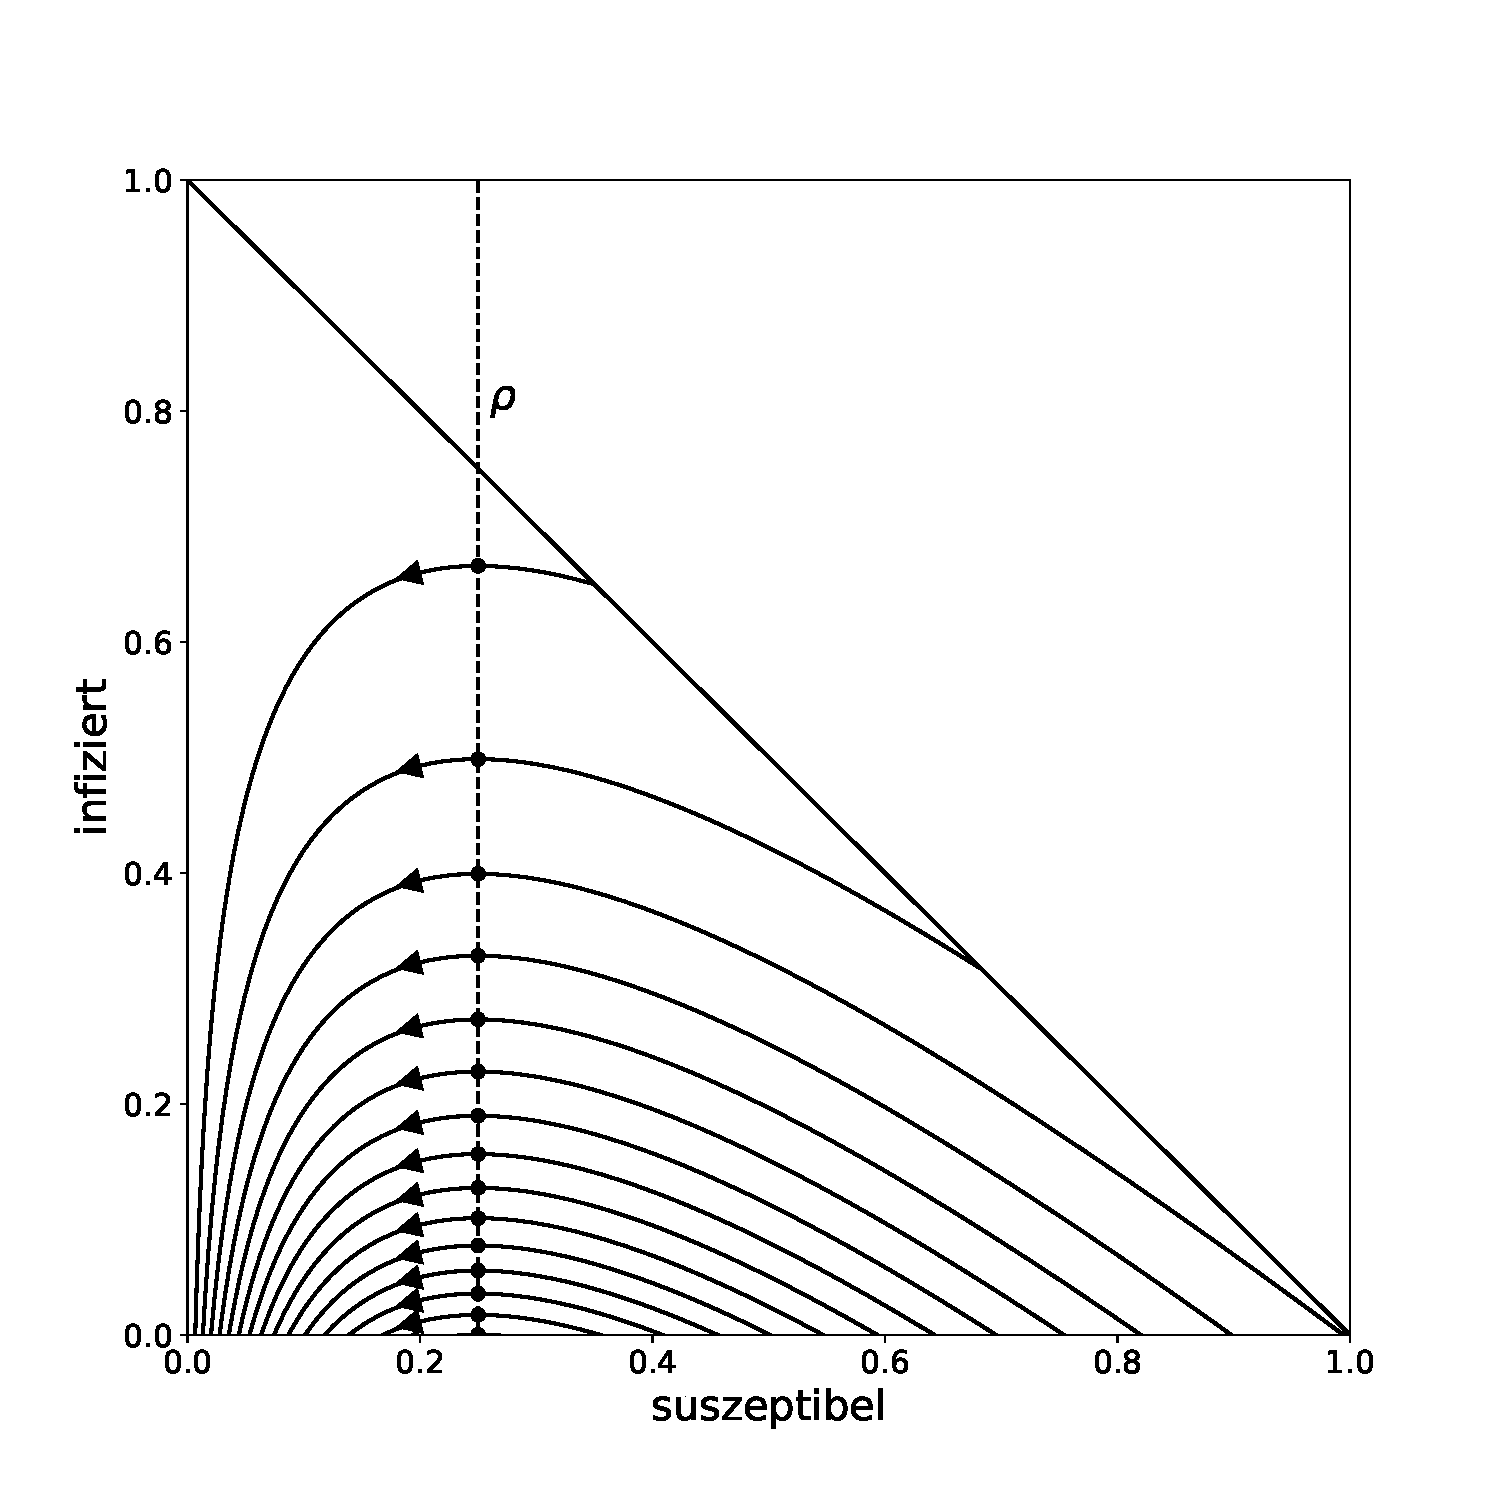
\includegraphics[width=\textwidth]{phase_portrait.pdf}
            \caption[Phasenportrait des SIR-Modells]{Phasenportrait der SI-Ebene des SIR-Modells mit den Parametern $\beta=2$ und $\gamma=0.5$}
            \label{fig:phase_portrait}
        \end{figure}

    \subsection{Bewertung der Aussagekraft des Modells}
    Vergleichen wir den Verlauf des SIR-Modells (Abbildung \ref{fig:sir}) mit der realen Entwicklung (Abbildung \ref{fig:covid19_incidence}), so erkennen wir zwei entscheidende Unterschiede:
    Der reale Verlauf von Covid-19 zeichnete sich durch mehrere Infektionswellen aus und die Krankheit ist noch nicht aus der Bevölkerung verschwunden.
    Da die Simulation von den beobachteten Daten abweicht, ist das SIR-Modell nicht aussagekräftig und die Annahmen müssen angepasst werden.

\end{document}
